\section*{Algoritmo de Karp-Rabin (o Rabin-Karp)}
\phantomsection
\addcontentsline{toc}{section}{Algoritmo de Karp-Rabin}

\phantomsection
\subsection*{Introducción del Algoritmo de Karp-Rabin}
% \addcontentsline{toc}{subsection}{Introducción del Algoritmo de Karp-Rabin}
\quad El algoritmo de Karp-Rabin es el único de los que estamos analizando que usa el método de hashing. Para esto utiliza un número primo alto y una formula para sacar el hash value del patrón y de las secciones del texto que se están evaluando. Al encontrar un valor de hash que coincida entonces va a evaluar si la sección que está evaluando en el momento es igual que el patrón, carácter por carácter. Esta es la razón por la cual se utiliza un primo grande, porque al depender de residuos (primo todos los números van a salir modulo si mismo porque el primo solo es modulo 0 con si mismo) si el número evaluando es más grande que el primo entonces puede dar el mismo valor para lo que no debería.


\phantomsection
\subsection*{Implementación del Algoritmo de Karp-Rabin}
% \addcontentsline{toc}{subsection}{Implementación del Algoritmo de Karp-Rabin}

(Con ayuda de \cite{Cormen_Leiserson_Rivest_Stein_2009}, \cite{HakakSaqibIqbal2019ESMA}, \cite{KRGFG} y \cite{Karp-Rabin})

\begin{algorithm} [H]
    \caption{Algoritmo de Karp-Rabin}\label{alg:KR}
    \begin{algorithmic} [1]
        \Procedure{karp\_rabin}{(patron, texto)}
            \State $n = len(patron)$
            \State $m = len(texto)$
            \State $d = 256$ \Comment{Este es el alfabeto defecto que sale en varios analisis (caracteres alfabeto inglés)}
            \State $q = 33554393$ \Comment{Cualquier número primo sirve, pero preferiblemente alto porque los pequeños solo hacen que el algoritmo corra como fuerza bruta porque más hashes concuerdan}
            \State $h = d^{m-1} mod(q)$
            \State $ValorHashPatron = 0$
            \State $ValorHashVentanaTexto = 0$
            \State $listaIndices = []$

            \For{i = 0 < n}
                \State $ValorHashPatron = (d*ValorHashPatron + patron[i]) mod(q)$ \Comment{Esta operación sirve con un abecedario normal como tabla ascii, para usarlo en Python el accesor se tiene que meter como parametro de ord()}
                \State $ValorHashVentanaTexto = (d*ValorHashVentanaTexto + texto[i]) mod(q)$
            \EndFor

            j = 0 \Comment{definirla afuera para poder usarla dentro del for sin tener que redefinirla cada vez que empiece el for otra vez}
            \For{$i = 0 \leq m-n$}
                \If{ValorHashPatron == ValorHashVentanaTexto} \Comment{Solo hacer fuerza Bruta cuando los valores hash concuerdan}
                    \For{$j = 0 < n$}
                        \If{$patron[j] != texto[i+j]$} \Comment{Si la fuerza bruta se incumple salga}
                            \State break
                        \Else
                            \State $j += 1$
                        \EndIf
                    \EndFor
                    \If{$j == n$}
                    \State $listaIndices += [i]$ \Comment{Al llegar al final de la fuerza bruta regista el indice}
        \EndIf
    \EndIf 
    \If{$i < m - n$}
        \State $ValorHashVentanaTexto = (d * (ValorHashVentanaTexto - texto[i] * h) + texto[i + n]) mod(q)$
        \If{$ValorHashVentanaTexto < 0$} \Comment{GeeksForGeeks recomienda en caso de que den hashes negativos}
            \State $ValorHashVentanaTexto += q$
        \EndIf
    \EndIf
\EndFor
\State return listaIndices

\EndProcedure
                    % \algstore{kr}

    \end{algorithmic}
\end{algorithm}

% \begin{algorithm}[H]
%     \begin{algorithmic}[1]
%         \algrestore{kr}
        
%     \end{algorithmic}
% \end{algorithm}


\phantomsection
\subsection*{Análisis del Algoritmo de Karp-Rabin}
% \addcontentsline{toc}{subsection}{Análisis del Algoritmo de Karp-Rabin}

\subsubsection*{Paso 1: Establecer el tamaño n de los datos}
% \addcontentsline{toc}{subsubsection}{Paso 1: Establecer el tamaño n de los datos}
Las dos variables que varían el tamaño de datos es la cantidad de caracteres del patrón $n$ y la del texto $m$. Entonces termina siendo $len(patrón) + len(texto) = n + m$

\subsubsection*{Paso 2: Determinar las operaciones de interés}
% \addcontentsline{toc}{subsubsection}{Paso 2: Determinar las operaciones de interés}
Las operaciones de interés son las comparaciones tanto del valor de hash como el carácter y van a contar como 1.

\subsubsection*{Paso 3: Encontrar los casos base}
% \addcontentsline{toc}{subsubsection}{Paso 3: Encontrar los casos base}
El algoritmo tiene tres sub-ecuaciones el de tiempo que tarda comparar los caracteres de patrón, los caracteres de texto y las comparaciones de los hashes.
\[T_{patrón}(0) =  0\]
\[T_{patrón}(1) = 1\]

\[T_{patrón}(n) = 1 + T_{patrón}(n-1)\]

\[T_{texto}(0) =  0\]
\[T_{texto}(1) = 1\]

\[T_{texto}(m) = 1 + T_{texto}(m-1)\]

\[T_{hashes}(0) = 0\]
\[T_{hashes}(1) = 1\]
\[T_{hashes}(m) = 1 + T_{hashes}(m-1)\]


\[T_{Karp-Rabin}(n,m) = T_{hashes}(m) + T_{texto}(m) * T_{patrón}(n)\]

Se hace de esta manera porque siempre se evalúan los hashes y después por aparte se hace un fuerza bruta de la sección.
\subsubsection*{Paso 4: Evaluando la ecuación recursiva}
% \addcontentsline{toc}{subsubsection}{Paso 4: Evaluando la ecuación recursiva}

\[T_{patrón}(n) = 1 + 1 + 1 + 1 ... + 1 + 1\]

\[T_{patrón}(n) = n \]

\[T_{texto}(m) = 1 + 1 + 1 + 1 ... + 1 + 1\]

\[T_{texto}(m) = m \]

\[T_{hashes}(m) = 1 + 1 + 1 + 1 ... + 1 + 1\]

\[T_{hashes}(m) = m \]

\[T_{Karp-Rabin}(n,m) = m + m * n\]

\subsubsection*{Paso 5: O-grande}
% \addcontentsline{toc}{subsubsection}{Paso 5: O-grande}

Dado a lo que evaluamos en los últimos pasos se sabe que O-grande es $O(m) + O(m*n) \sim O(m*n)$

Es importante notar que ese tiempo ocurre cuando todos los caracteres son lo mismo entonces tiene que evaluar todos los caracteres. El tiempo normal es $O(m) + O(cn) \sim O(m+n), c$ constante.


\subsubsection*{Paso 6}
% \addcontentsline{toc}{subsubsection}{Paso 6}
\begin{figure} [H]
    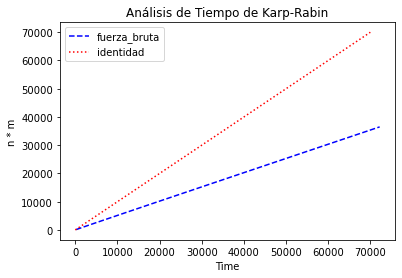
\includegraphics[width=0.5\textwidth]{../codigoPythonJupyter/rk/Final.png}
    \caption{Karp-Rabin (Anexo rabinkarp.ipynb)}
    \label{fig:kr}
\end{figure}
